\subsection{Sidechain Scheme}
\label{sec:side}


\subsubsection{Plasma}
\noindent As the second-layer expansion framework of Ethereum, Plasma has been proposed by \textsc{Joseph Poon} (founder of Lightning Network) and \textsc{Vitalik Buterin} (founder of Ethereum) in 2017 \cite{poon2017plasma}. The first thing to be clear is that Plasma is essentially a set of frameworks instead of a separate project. It provides an off-chain solution for a variety of different project real projects. \\
\noindent Layer 2 expansion of blockchains often known as off-chain expansion, similar to lightning network, this kind of expansion scheme does not need to modify the underlying protocol of the blockchain, but by transferring a large amount of frequent calculation work "off-chain", and submitting the calculation results to the "main chain" guarantee its finality as we discussed previously. Plasma works like blockchains in blockchains where anyone can create different Plasma on top of the underlying blockchain to support different business needs. \\
\noindent As an example of sidechain, Plasma derived from the general concept of symmetric 2-way pegged scheme to realize the transfer solution. The overall process of asset exchange is shown in figure \ref{fig:2way}. 
        \begin{figure}[H]
        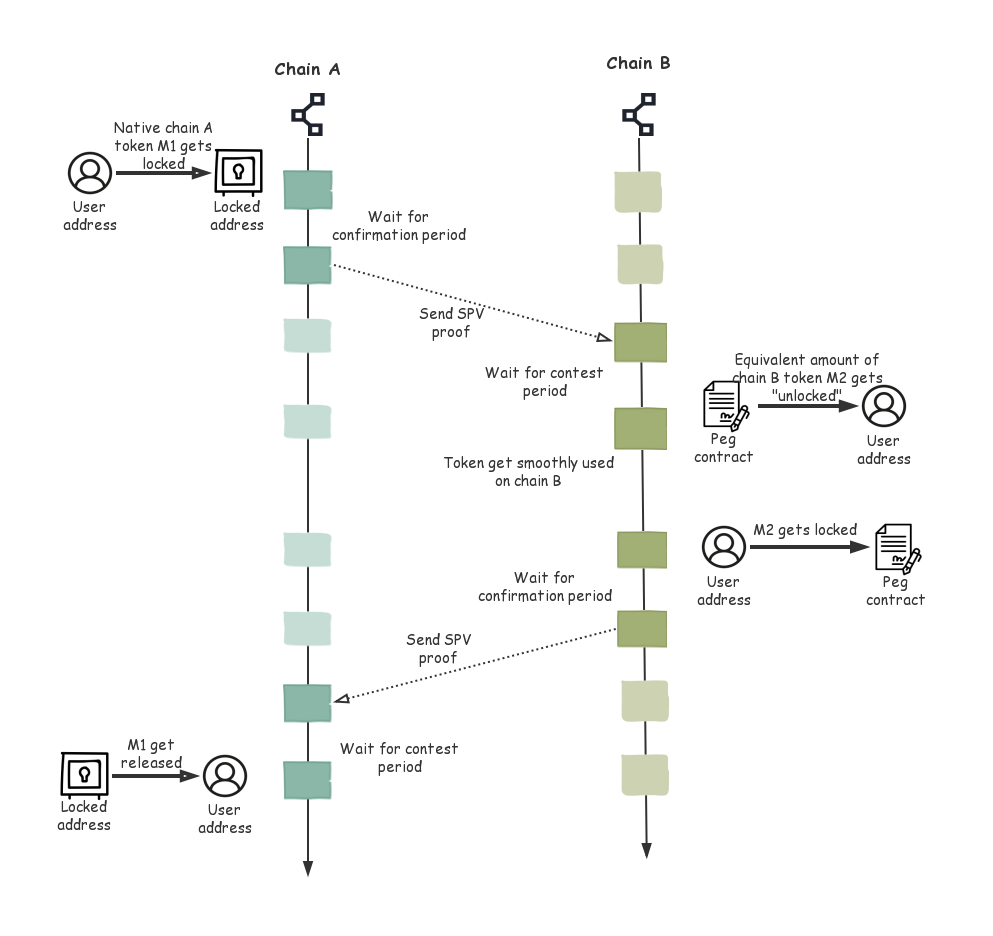
\includegraphics[width=1\textwidth]{./figures/2way.png}
        \centering
        \caption{{2-way pegged sidechain diagram}\protect\footnotemark}
        \centering
        \label{fig:2way}
        
        \end{figure}
\footnotetext{SPV to verify that the transaction exists (recognized by other nodes on the blockchain)}
\begin{enumerate}
    \item When chain A wants to transfer the asset to chain B, it first needs to initiate a transfer transaction Tx1 (chain A's locking addr1 + chain B's receiving address addr2), and the asset M1 is locked on the addr1.
    \item After Tx1 transaction is submitted, it is necessary to wait for a \textit{confirmation period} so that there are enough blocks and calculations to ensure that the cross-chain transaction Tx1 is confirmed, reducing the impact of refactoring on cross-chain transactions.
    \item After the confirmation period, the \textbf{SPV} certificate containing Tx1 will be sent to chain B. B knows that chain A has indeed initiated and locked asset M1, so it generates a corresponding amount of M2 on chain B according to a certain ratio. The value of M1 is transferred to M2 means the assets on chain A are transferred to chain B.
    \item After M2 is generated on B, it is necessary to wait for the \textit{competition period} before unlocking M2 to avoid double-spend attack in chain A reconstruction.
    \item After unlocking, M2 can freely circulation on chain B.
    \item The process of a transaction from chain B to chain A is similar to previous steps.
\end{enumerate}
\noindent Plasma supports multi-level sidechains and uses MapReduce mode to perform parallel computing, which greatly improves sidechain performance. The block header and hash data of the side chain will be sent to the main chain, and \textit{Proof of Fraud} can be used to ensure the correctness of the sidechain transaction.


\subsubsection{Liquid}
\noindent Liquid\cite{Liquid} is a sidechain of BTC and a typical representative of the multi-signature notary mechanism. It is designed to meet the BTC fast transfer needs of exchanges, market makers and brokers. Therefore, Liquid uses the multi-sig federation mechanism to confirm the transaction block, which can greatly improve the transaction speed.\\
\noindent Liquid based on Element codebase and uses Strong Federation technology to support 1:1 Bitcoin exchange. The basic process of the transaction is described as Figure \ref{fig:multisig}. The confirmation of this asset transfer requires multi-signature from the majority of notaries.

        \begin{figure}[H]
        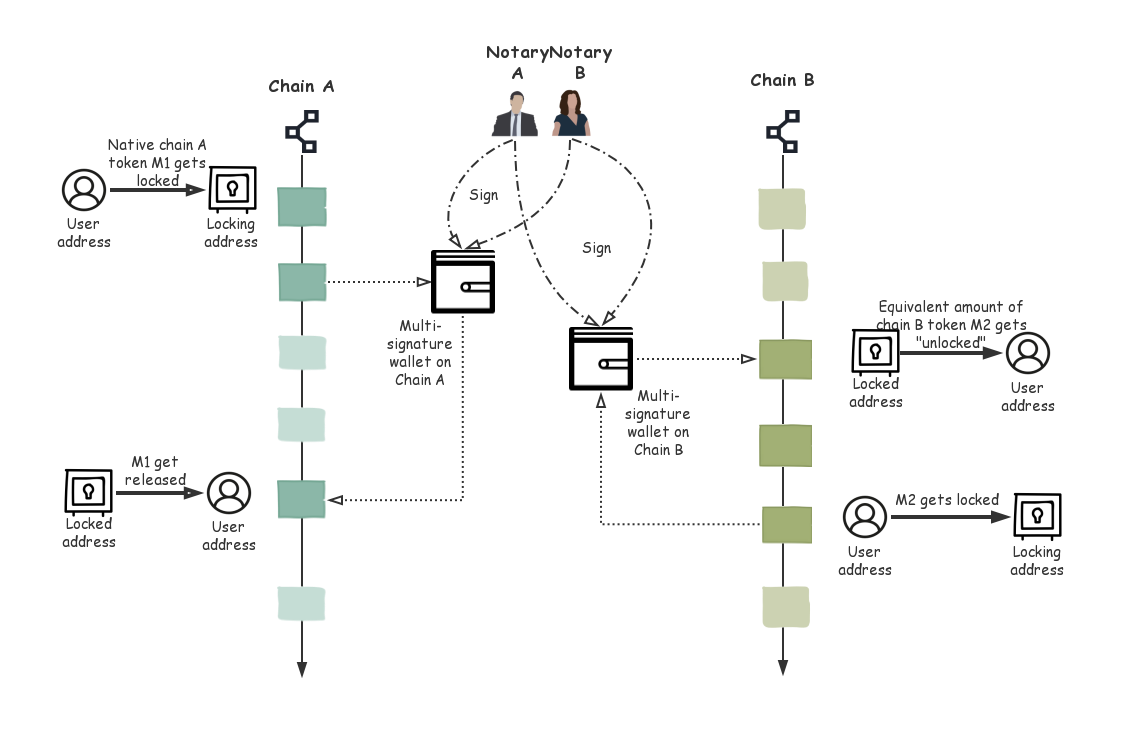
\includegraphics[width=1\textwidth]{./figures/multi_sig.png}
        \centering
        \caption{Multi-signature federation scheme}%\protect\footnotemark}
        \centering
        \label{fig:multisig}
        \end{figure}
        
\noindent In Strong Federation, there are 2 types of node role in the network:
\begin{itemize}
    \item Blocksigners: Signature verification for transactions in the sidechain to achieve block consensus. 
    \item Watchmen: When the asset is transferred from the sidechain to the main chain, it is responsible for signature verification of the transaction on the main chain, indicating that the sidechain asset has indeed been destroyed, and the main chain can unlock the corresponding number of assets.
\end{itemize}

\subsubsection{Elastos}
\noindent In order to ease the pressure on the main chain as well as provide better user experience for DApps, Elastos\cite{Elastos} adopted the main chain + sidechain architecture,  main chain only responsible for the circulation of the ELA while the DApps run on the sidechain. \\
\noindent In this scenario, the transfer of the assets between the main chain to sidechain is in a one-to-many relationship. It is feasible that the side chain only saves all the block header information of the main chain. If the main chain needs to save the block header information of all the side chains, it will lead to poor scalability. So Elastos uses asymmetric 2-way peg scheme based on SPV to realize the cross-chain function.\\
\noindent Assets from the main chain to the sidechain, Elastos using SPV proof to prove the transactions, while it secures the transfer using multi-signature notary scheme when transfer from sidechain to the main chain. We can regard this process as a combination of Plasma and Liquid.

\subsubsection{OneLedger}
\noindent As one cross-chain consensus protocol, OneLedger\cite{Oneledger} uses sharding and improved practical Byzantine fault-tolerant consensus. By creating sidechain, it can easily realize cross-chain interactions between individuals or business in OneLedger. OneLedger defines a three-layer consensus protocol to integrate different blockchain applications more efficiently.\\
\noindent Different from what we have discussed before, OneLedger as a sidechain, it realizes the synchronization of assets and values between the main chain and sidechain by applying multi-sig federation and drive-chain.\\
\noindent A drivechain\cite{lerner2016drivechains} gives custody of the locked coins to the miners, allowing them to (algorithmically) vote on when to unlock coins and where to send them. As Figure \ref{fig:drive} shows:
        \begin{figure}[H]
        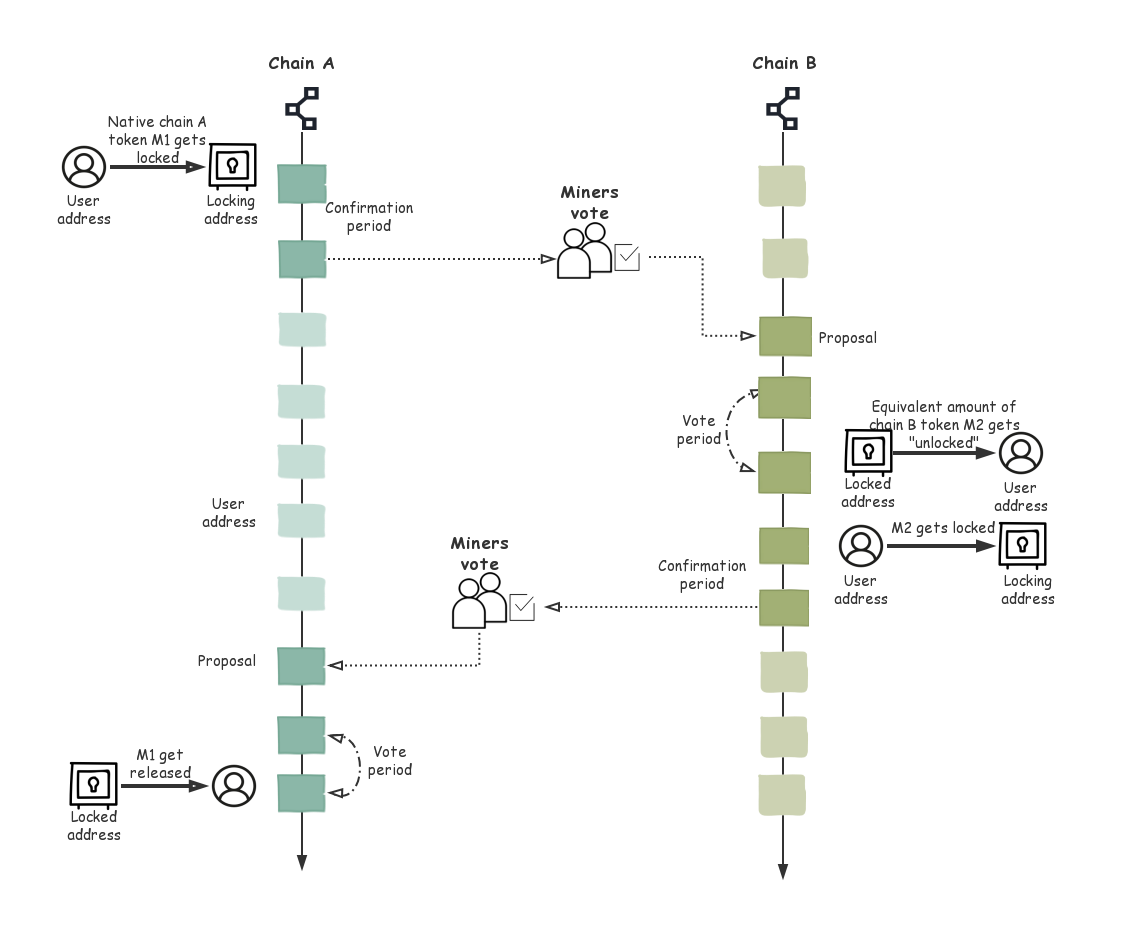
\includegraphics[width=1\textwidth]{./figures/drive.png}
        \centering
        \caption{Drivechain  working diagram}%\protect\footnotemark}
        \centering
        \label{fig:drive}
        \end{figure}
\noindent According to OneLedger's white paper, the core of OneLedger is a set of consensus protocols that enable OneLedger to effectively integrate different blockchain products. As far as I understand that the protocol mentioned here is not a specific consensus protocol algorithm in the traditional sense, but a series of concepts and application scenarios. Among all 3 layers, I specifically studied the \textit{Public Chain Consensus} which apply on the atomic transfer between blockchains through OneLedger Network on the base layer.
        \begin{figure}[H]
        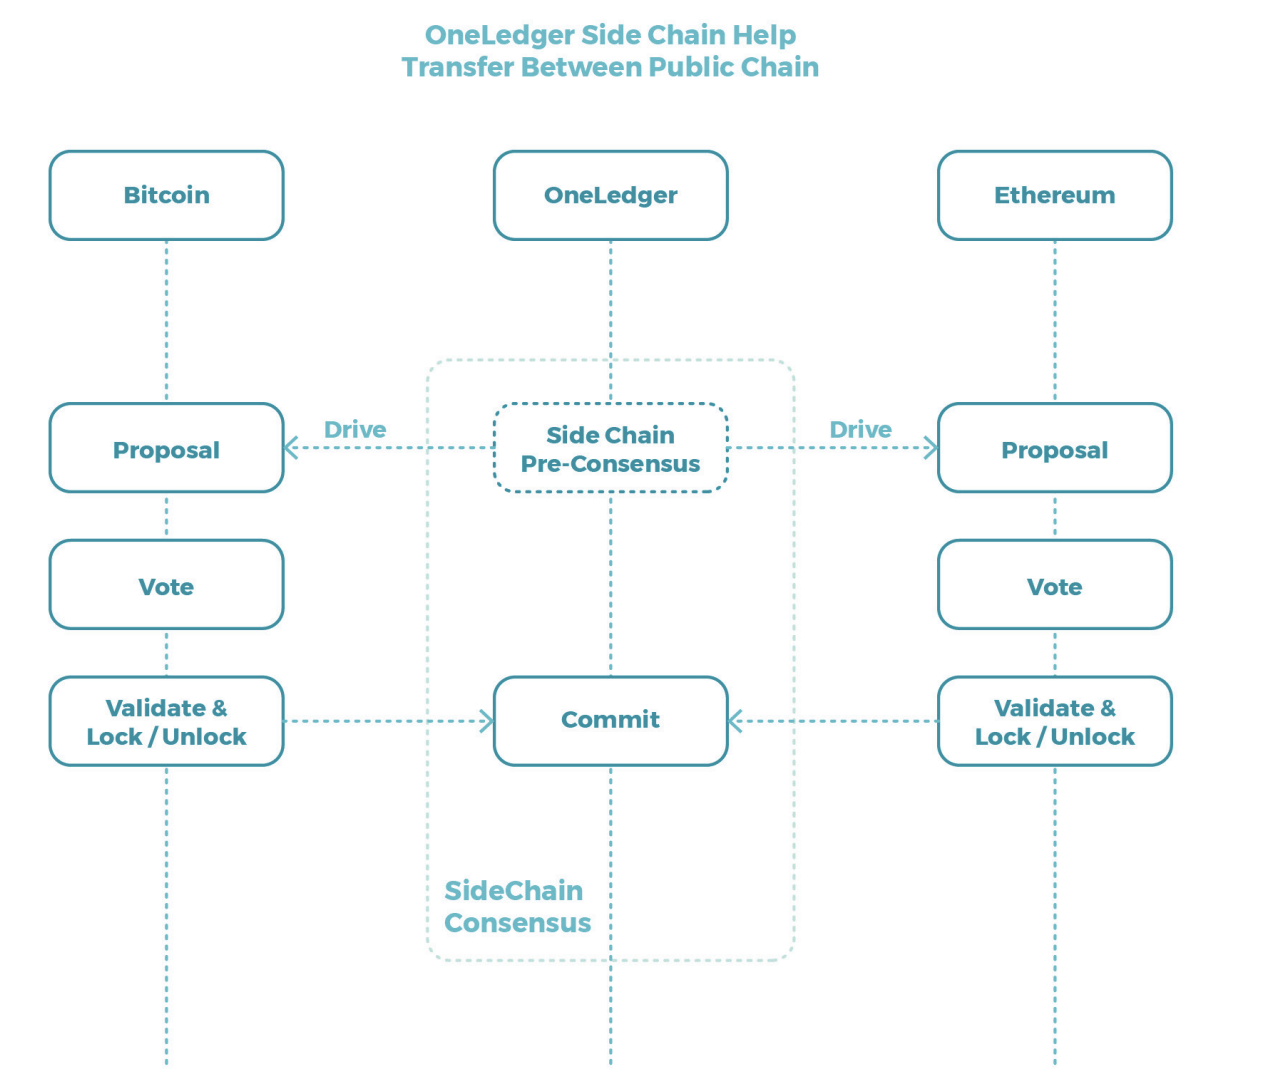
\includegraphics[width=1\textwidth]{./figures/oneledger.png}
        \centering
        \caption{{OneLedger sidechain architecture}\protect\footnotemark}
        \centering
        \label{fig:oneledger}
        
        \end{figure}
\footnotetext{Image courtesy of OneLedger white paper\cite{Oneledger}}
\noindent There's 2 steps in sidechain consensus algorithm:
\begin{itemize}
    \item \textbf{Round base pre-consensus}: Use to obtain a consensus proposal with more than 2/3 participants' votes.
    \item \textbf{Commit}: When the purposed block has reached a pre-consensus stage, it needs to drive to the public chain when necessary, and accepts the verification process. Once the proposal is accepted by both public chains, the new block will be officially “committed” to the OneLedger network, and once more than 2/3 of the participants complete the commits, the block is finalized. 
\end{itemize}